\documentclass[11pt]{ujarticle}\sloppy
\usepackage{funinfosys}
\usepackage[hyphens]{url}
\usepackage[dvipdfmx]{graphicx}
\author{% 
b1021204 西侑亮\\指導教員 : 松原克弥
}		
\course{Informalstion Systems Course}

\title{独自管理インターフェースを持つ未来大クラウドシステムのIaC対応}
\etitle{FUN Cloud System Which Have Unique Management Interface
\\Implementatios of IaC}
\eauthor{Yusuke Nishi}
\abstract{今日の多くの大学では,プログラミング実行環境を提供するクラウドシステム導入が加速している.
クラウドシステムによる仮想マシンを用いることで,多様な端末上で統一された実行環境を用意できるようになった.
しかし,仮想マシンの作成や設定を学生人数分用意するためには多くの手順を必要とするが課題である.
クラウドシステムをコードで管理する手法であるInfrastructure as Code(IaC)に対応させることで効率的に管理することが期待できる.
本研究では,公立はこだて未来大学(以降,未来大)にて使用されているクラウドシステムをIaCに対応させることにより,効率よく統一環境を用意し,講義の効率化を目指す.
}
\keywords{クラウドシステム, IaC, 公立はこだて未来大学}
\eabstract{
	Nowadays, the number of university is include which use cloud systems for programming develop environment.
	Virtual machines based on cloud systems can be prepared a unified development environment in deferent machines. However, the problem is that many processes are needed to create and configure virtual machines for the number of students. Using of Infrastructure as code (IaC) that the approach of managing Cloud systems by code can be expected to manage efficiently.The study's goal is to improve seminar efficiency by efficiently constructing a unified development environment for the cloud system used at Future University Hakodate (FUN) that is compatible with IaC.
	}

\ekeywords{Cloud System, IaC, Future University of Hakodate}
\begin{document}
\maketitle


\section{背景と目的}
\label{sec:intro}
近年,情報科学分野を専攻とする大学や高等専門学校における演習講義において,学生人数分のPCを設置して統一された演習環境を用意する授業スタイルから,
学生個人がPCを用意するBYOD(Bring Your Own Device)へと変化している\cite{byod}.BYODにおいて学生が所有するPCのOSや内部設定が異なる.
%なぜ統一環境?BYODについても述べる
そのため,未来大や大阪大学では,クラウドシステムを利用して仮想マシンを用いて統一された演習環境を提供している\cite{oosakadai}.


クラウドシステムを利用する事例が増加するとともに,新たな課題も浮上している.
仮想マシンの作成,設定にあたり授業時間や教員の手間が必要となることである.
例えば,未来大における情報科学の演習講義の一つである並列分散処理では,複数台の仮想マシンを用意して一つのプログラムを並列分散実行する演習がある.
2023年度に行われた同科目では未来大クラウドシステムでの実行方法やマシンの初期設定について合計10ページにわたる解説が行われている.
講義を受講している学生分の仮想マシンの準備にかかる手順を短縮することができれば,授業の効率向上を見込める.

%目的

本研究は,演習用クラウドシステムのIaC対応について実装・評価を行う.
IaCとは,プログラミング言語で書かれたコードを実行することによりITインフラストラクチャを作成管理する手法のことを意味する\cite{O'Reilly Media}.
Micheleら\cite{InformationSystem}は,IaCを用いることで次のような利点をもたらすと述べている.コードを配布することにより,仮想環境構築の再現と再利用が容易にできるようになる.
また,手作業による手順が減少し,環境構築の効率性が向上する.
演習用クラウドシステムをIaCに対応させることにより,コードで仮想マシンを管理することが可能となる.
さらに,コードを配布し実行するのみで実行環境を再現できる.
従来多くのスライドを用いて説明する必要がなくなり,授業効率の向上が見込める.
演習用クラウドシステムのIaC対応を実現し講義の効率化を目指す.


\section{Terraform}


本研究では,IaCフレームワークの一つであるTerraformをもちいる.数多あるIaCフレームワークの中からTerraformを選んだ理由として,
デファクトスタンダードである,つまり利用者がもっとも多く,対応するクラウドプロバイダが多いことを挙げる.
TerraformはAmazon Web Services(以降,AWS)や
Microsoft Azure,Google Cloud Platformなどのクラウドプロバイダに対応しているため,
Terraformのコードを学習することで多くのプロバイダーを同様のコマンドで管理することができる.
さらに,Terraform Custom Framework Providerという,新規にクラウドシステムをTerraformに対応させるプログラムが公開さている.
Terraform Custom Framework ProviderはGo言語で記述されたプログラムであり,対応させたいクラウドシステムに合わせて書き換えることでTerraform対応を実現する.
作成したTerraform Custom Framework ProviderはTerraformを介して,世界中に公開することも可能である.
また,プロビジョニング機能を備えている点も理由に挙げる.プロビジョニング機能とは仮想マシンの作成・起動時にデータベース,キャッシュ,ロードバランサ,キュー,サブネットの設定などの仮想マシンの環境設定を行う機能である.
Terraformでは仮想マシン作成・起動後にマシンに対してSSH接続を行いプロビジョニング機能を実現している.


\begin{figure}[h]
	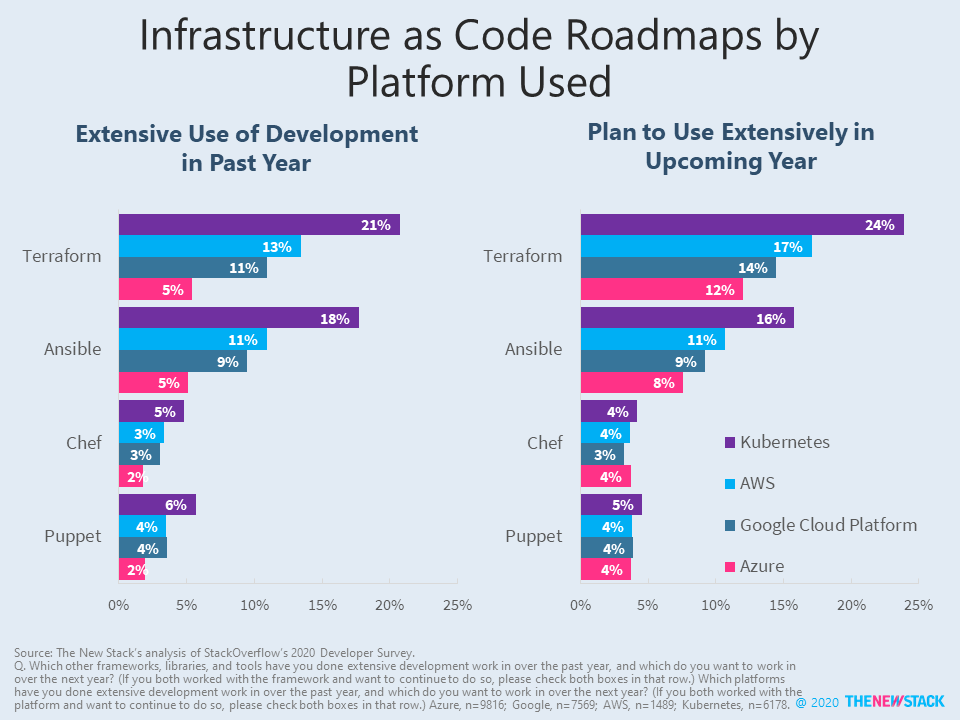
\includegraphics[width=1\linewidth]{./images/terraform.png}
	\caption{2020年のIaCプラットフォームの利用率比較\cite{THENEWSTACK}}
	\label{fig:terraform}
\end{figure}


本研究では,未来大クラウドシステム用のTerraform Custom Framework Providerを用意し,Terraform に対応させることで仮想マシンを管理する手法を確立する.
Terraformに対応させるためには,クラウドシステム管理に用いるApplication Programming Interface(以降,API)が公開されている必要がある.
しかし,未来大クラウドシステムではAPIが公開されていない.公開されていない理由として以下の理由が挙げることができる.
未来大クラウドシステムでは,学生がアカウント認証をして,学生がそれぞれの仮想マシン管理画面(WebAPI)へと遷移する.その後,マシン作成や起動,停止,削除を行う.
一見,学生それぞれのアカウントが独立してクラウドシステムを管理しているように見えるが,未来大クラウドシステム内部では全てのアカウントの管理要求を集約し,一つのAWSアカウントが管理している.
そのため,アカウントひとつひとつに対して,個別にAPIを公開するためには,システムの大幅な改変が不可欠であり,多くの労力と費用を要する.


\begin{figure}[h]
	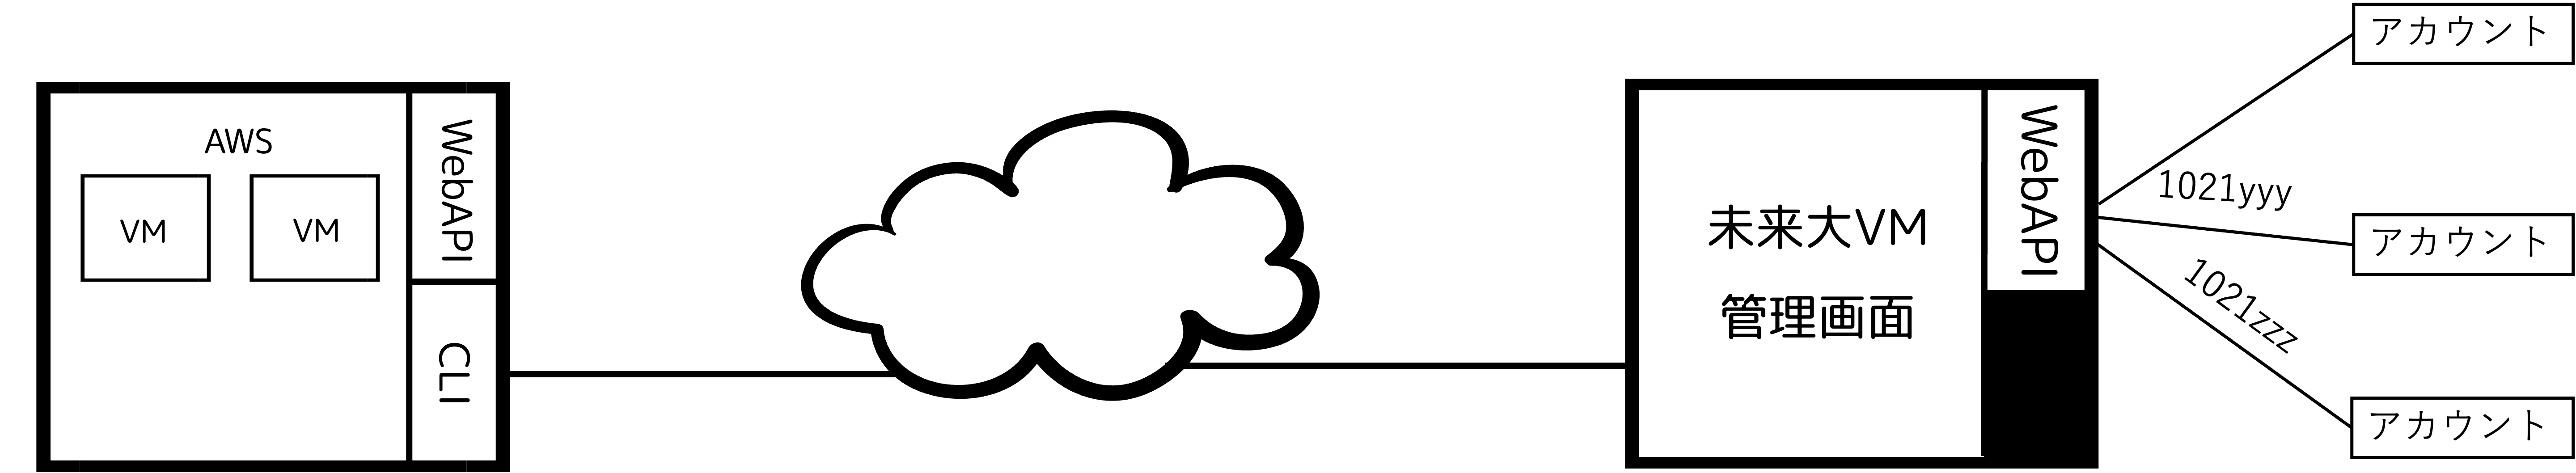
\includegraphics[width=1\linewidth,height=2cm]{./images/cloud.png}
	\caption{未来大クラウドシステムの構造}
	\label{fig:cloud}
\end{figure}



\section{スクレイピング}


本研究では,APIを用いるのではなく,スクレイピングを用いた操作により,未来大クラウドシステムの操作を実現する.
スクレイピングとは,WEBページ上のHTMLやCSSに存在するタグやデータ構造を解析し.構造化されているデータをプレーンなデータへと抽出し変換する技術である.
スクレイピングはプログラムを使用して行われ,目的のWeb ページのHTMLデータを解析し,特定の情報をユーザからのリクエストに応じて自動的に取り出すことを可能にする.
スクレイピングは,データ解析,機械学習,市場調査,自動化テスト,自動入力など,多様な分野で使用されており,データ収集手段として注目を浴びている.
ログイン認証が必要なページや,フォーム入力が必要な場合にも,スクレイピング技術は有効であり,このような場合,ヘッドレスブラウザや専用のライブラリを使用し,自動的にフォームを入力,ログインプロセスを完了させることができる.
スクレイピングを活用し,未来大クラウドシステムのWebAPIを自動で操作することにより,未来大クラウドシステムの操作を実現する.


\begin{figure}[h]
	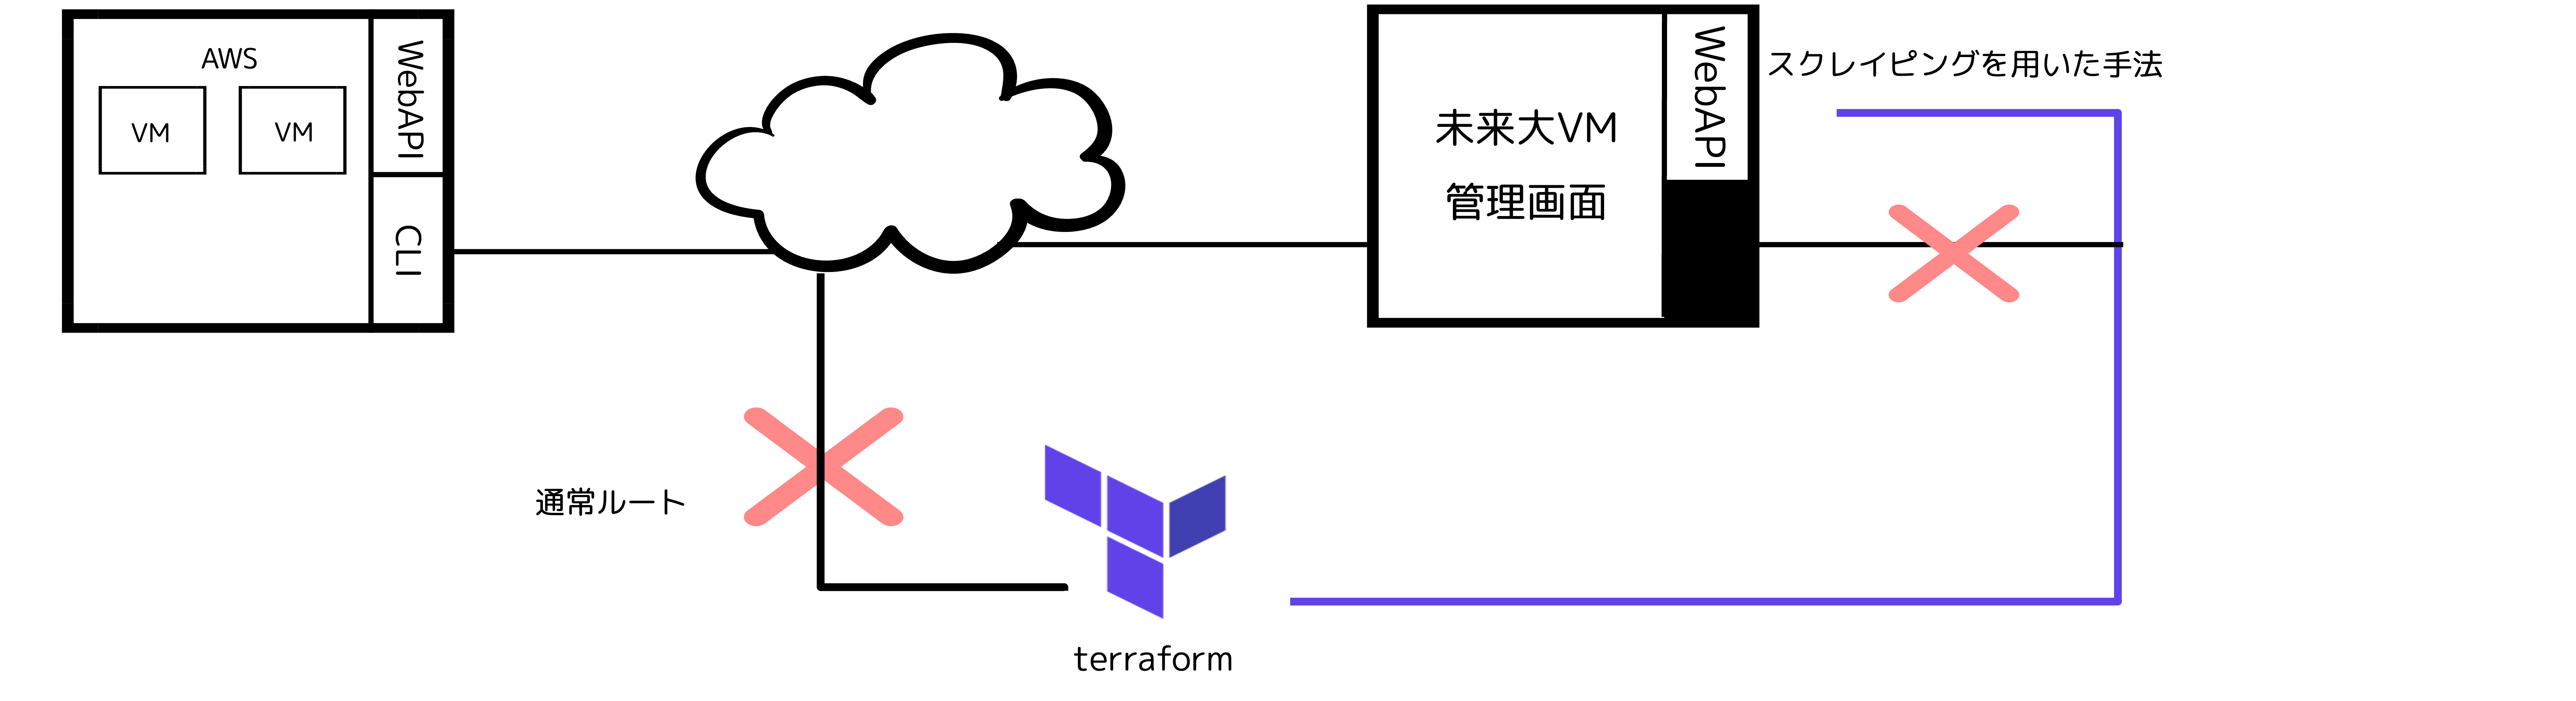
\includegraphics[width=1\linewidth]{./images/scraping.png}
	\caption{スクレイピングによる未来大クラウドシステムの管理}
  \label{fig:scraping}
\end{figure}


%
%Agoutiとは,Web自動化に優れたスクレイピングツールで,ユーザーの動きを再現してブラウザを自動操作することに秀でている.
%また,ドロップダウンメニューの選択やボタンクリック,フォームへの自動入力を実行することが容易であり,
%ログイン認証への対応の操作に適している.また,AgoutiはGo言語上で使用可能なツールである.
%本研究で操作する未来大クラウドシステムのWebAPIはドロップダウンメニューによる選択やボタンクリックによる画面遷移,ユーザー認証が存在している動的なWebページである.
%また,Terraform Custom Framework ProviderはGo言語でプログラミングされていることから,本研究で用いるスクレイピングツールとしてAgoutiを採用する.
%

%Agoutiを動作させるWebDriverとして,ChromeDriverを採用する.WebDriverとは, Webページへの移動やユーザ入力などが可能なオープンソースフレームワークである.
%ChromeDriverはGoogleChromeを自動制御するためのWebDriverである.ChormeDriverはクロスプラットフォーム対応しており,様々なオペレーティングシステム上で動作する.
%また,Chromeブラウザの内部APIを直接利用しているため高速で動作する.本研究では,学生が所有するPC環境が異なっていても同様に動作することが望ましいため,ChromeDriverが適している.


\section{提案}


本研究は,未来大クラウドシステムをIaC対応化させることを提案する.
仮想マシンのコードを用いた管理と,コードの配布によるマシン環境の再現が可能となる.
従来の演習用仮想マシンの準備と比べ,大幅な時間短縮を期待できる.
クラウドシステムを直接操作するAPI使わず,
スクレイピングを用いて,WebAPIを操作することでIaC対応を実現する.


\section{実装}



本実装では,Terraformを用いてクラウドシステムを操作する際,仮想マシンの設定を記述したファイルを用意する.
未来大クラウドシステムを管理する際には、アカウント認証用のアカウント名,パスワード,演習環境の選択,管理するマシン名,マシンのスペック,マシンを停止させるかを記載する設計とする.


\begin{figure}[h]
	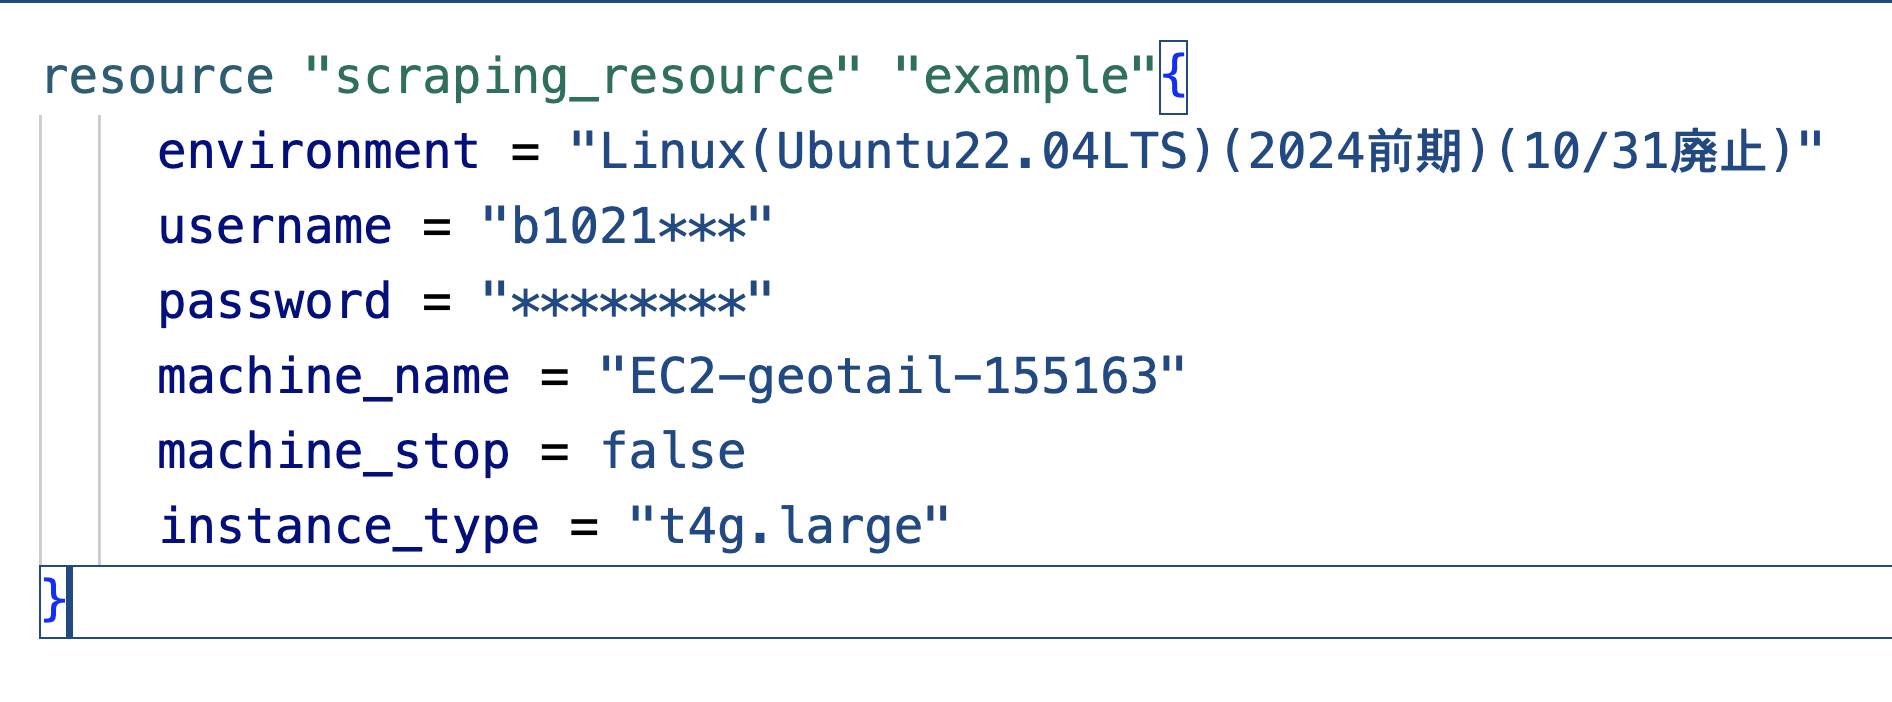
\includegraphics[width=1\linewidth]{./images/machine.png}
	\caption{設定ファイルの記述}
  \label{fig:machien}
\end{figure}


スクレイピングを用いて未来大クラウドシステムにアクセスすると,最初にユーザ認証画面へと遷移する.
ユーザー情報とパスワードをフォームに自動入力し,ボタンクリックを行うことで環境選択画面に遷移する.
環境選択では,年度や時期,受講している講義ごとに異なる環境を選択することが可能である.
設定ファイルで指定された環境選択と合致する文字列をドロップダウンから選択したのち,仮想マシン管画面へ遷移する.
仮想マシン管理画面では,作成,起動,停止,削除の機能がある.
さらに,仮想マシンの作成,起動時では,仮想マシンのスペックを変更することが可能である.
設定ファイルでマシン名を指定せずに,Terraformの仮想マシン起動コマンドであるterraform applyを実行された時に,マシンの新規作成を行う設計とする.
設定ファイルでマシン名を指定し,terraform applyを行うことで,停止中の仮想マシンを起動できるよう設計する.作成,起動処理時に設定ファイルに記載されたマシンスペックに合致したものを選択する.

プロビジョニング機能を用いる際,仮想マシンのパスワードやIPアドレス,秘密鍵が必要となる.パスワードやIPアドレスはスクレイピングによって,
HTMLから自動抽出する機能を実装する.秘密鍵はWebAPIをスクレイピングして自動でダウンロードし,ダウンロード先の絶対パスを返す機能を実装する.


設定ファイルにて,仮想マシンの停止を要求するように記述し,terraform applyを行うことでWebAPiの停止ボタンを操作することで仮想マシンの停止が行われるよう実装する.
また,Terraformの仮想マシン削除コマンドであるterraform destroyを実行することによりWebAPIの削除ボタンを操作し,仮想マシンの削除機能を実現する.


本研究では,スクレイピングを行う処理をクラウドコンピュータ上で行う.クラウドコンピュータ上で行うことによりGO言語の環境構築を
ユーザーのPCにインストールする必要がなくなり、Terraformを実行する環境に左右されにくくなる.



\section{評価手法}

本システムの有用性を確認するために,
評価項目として定量的評価と定性的評価による測定を検討している.
定量的評価では,システムの使用における実行時間,システムそのもののレスポンス時間や安定性などのパフォーマンスメトリクスを測定する.
定性的評価では,
未来大の2024年度後期の情報科学演習講義である並列分散処理の受講生を被験者として評価実験を行い,
アンケートを通じて被験者の使用感や満足度や要望,システムに対する意見を収集する.



\section{進捗と計画}

進捗状況として,スクレイピングを用いてTerraformによる未来大クラウドシステムの管理を実装が完了した.
現在,システムの実行環境に,GO言語やスクレイピングツールを
インストールする必要がある.
Go言語を用いる機能とスクレイピング機能を,
クラウドコンピューティング上での実行の実現に取り組み,
実行環境に依存しないシステムの構築を目指している.
今後の計画として,クラウドコンピューティング上での実装が終わった後,実際に未来大の学生に使用してもらい,フィードバックを元に機能改善を目指す.


\section{結言}

本研究では,独自の管理インターフェースを持つ未来大クラウドシステムのIaC対応により,演習講義における統一環境準備の効率化を目指す.
クラウドシステムを直接管理することが困難なインターフェースのため,スクレイピングを用いて管理を行う.
今後の課題として,実行者のPC環境に依存しないように実装し,評価実験を行いたい.


\section{情報システムコースにおける本研究の位置づけ}

本研究では,スクレイピングにより学内クラウドシステムをIaCに対応させることによって,演習講義に用いる統一環境準備の効率化を目標としている.これは,未来大での演習講義を情報システムによって支援するものであり,効率性と信頼性を考慮した情報システムの実現と言える.今後,実装したシステムを評価実験を行うことで,カリキュラムポリシーの「結果の評価を通じて,新しい方法論や学問領域を切り拓く能力を育む」ことに繋がる.

\begin{thebibliography}{99}
	\bibitem{byod}
	大学ICT推進協議会: ICT利活用調査部会, "BYOD を活用した教育改善に関する調査研究 結果報告書", AXIES 大学ICT推進協議会.[Online]. Available from : \url{https://axies.jp/report/ict_survey/2016survey/}. Accessed: 2024-10-25.

	\bibitem{oosakadai}
	大阪大学, "大阪大学キャンパスクラウドサービス", 大阪大学. [Online]. Available from: \url{https://ccc.osaka-u.ac.jp/hosting/}. Accessed: 2024-10-21.
	\bibitem{O'Reilly Media}
	K. Morris: "Infrastructure as Code", O'Reilly Media, 2016.
	\bibitem{InformationSystem}
	Michele Chiari, Bin Xiang, Sergio Canzoneri, Galia Novakova Nedeltcheva, Elisabetta Di Nitto, Lorenzo Blasi, Debora Benedetto, Laurentiu Niculut, Igor Škof : "DOML: A new modeling approach to Infrastructure-as-Code", Information Systems, Volume 125, November 2024. 
	\bibitem{THENEWSTACK}
	B. Cameron Gain: "Terraform 1.0 Reflects What HashiCorp Has Learned About Infrastructure-as-Code", THENEWSTACK, [Online]. Available from: \url{https://thenewstack.io/terraform1-0-reflects-what-hashicorp-has-learned-about-infrastructure-as-code/?utm_referrer=https%3A%2F%2Fwww.google.com%2F/}. Accessed: 2024-10-22.
	%\bibitem{selenium}
	%SeleniumHQ, "Selenium Documentation", Selenium, 2023. [Online]. Available from: \url{https://www.selenium.dev/documentation/en/}. Accessed: 2023-10-25.
\end{thebibliography}
\end{document}
%
%
% EOF 

